% =====================================================================
%  Chapitre 5 -- CNN au-dela de la classification
%  Partie a : detection d'objets, segmentation, encodeur-decodeur, U-Net
% =====================================================================
\section{Chapitre 5 --- CNN au-delà de la classification}

\chapterslide{Chapitre 5}{CNN au-delà de la classification}%
{5 h --- détection d'objets, segmentation, CNN 1D, autres modalités}%
{\textbf{Objectifs.} Étendre le CNN au-delà de l'étiquette unique : localiser des objets
(boîtes englobantes, IoU, NMS), attribuer une classe à chaque pixel (segmentation sémantique,
par instance, panoptique), comprendre l'architecture encodeur-décodeur et les connexions
sautées de U-Net, et appliquer les mêmes principes aux \textbf{séries temporelles} avec un
noyau de convolution 1D.}

\begin{frame}{Plan du chapitre}
\begin{columns}[t]
\begin{column}{0.48\textwidth}
\begin{kbox}[Les quatre temps de ce chapitre]
\begin{enumerate}
  \item La \textbf{détection d'objets} : localiser \emph{et} classer.
  \item Les deux familles de détecteurs : une ou deux étapes.
  \item La \textbf{segmentation} : sémantique, par instance, panoptique.
  \item Les \textbf{CNN 1D} et les autres modalités.
\end{enumerate}
\end{kbox}
\end{column}
\begin{column}{0.48\textwidth}
\begin{ebox}[Ce que vous saurez faire]
\begin{itemize}
  \item Expliquer la différence entre classer, localiser et segmenter.
  \item Calculer un IoU et justifier une suppression des non-maxima.
  \item Décrire l'apport des connexions sautées de U-Net.
  \item Adapter un CNN 2D à un signal 1D (ECG, trafic).
\end{itemize}
\end{ebox}
\end{column}
\end{columns}
\vspace{1mm}
\begin{wbox}[Le fil rouge]
Classer, c'est répondre « \emph{quoi} ? ». Détecter, c'est répondre « \emph{quoi} et
\emph{où} ? ». Segmenter, c'est répondre « \emph{quoi}, pour \emph{chaque pixel} ? ».
Le même réseau convolutif sert aux trois : seule la \textbf{tête de sortie} change.
\end{wbox}
\end{frame}

\begin{frame}{De la classification à la localisation}
\begin{columns}[t]
\begin{column}{0.52\textwidth}
\centering
\end{column}
\begin{column}{0.45\textwidth}
\begin{itemize}
  \item \textbf{Classification} : une étiquette pour \emph{toute} l'image
  (« chien »).
  \item \textbf{Détection} : une ou plusieurs \textbf{boîtes englobantes},
  chacune avec sa classe et un score.
  \item \textbf{Segmentation} : une classe attribuée à \emph{chaque pixel},
  ce qui produit un \textbf{masque} de la même taille que l'image.
  \item La sortie change de forme : un vecteur, puis une liste de boîtes,
  puis une image de labels.
\end{itemize}
\end{column}
\end{columns}
\vspace{0.5mm}
\begin{kbox}[La question posée par chaque tâche]
\emph{Quoi ?} --- classifier. \quad \emph{Quoi et où (approximativement) ?} --- détecter.
\quad \emph{Quoi, pixel par pixel ?} --- segmenter.
\end{kbox}
% [fix] figure sortie
\end{frame}

\begin{frame}{De la classification à la localisation --- la figure}\begin{center}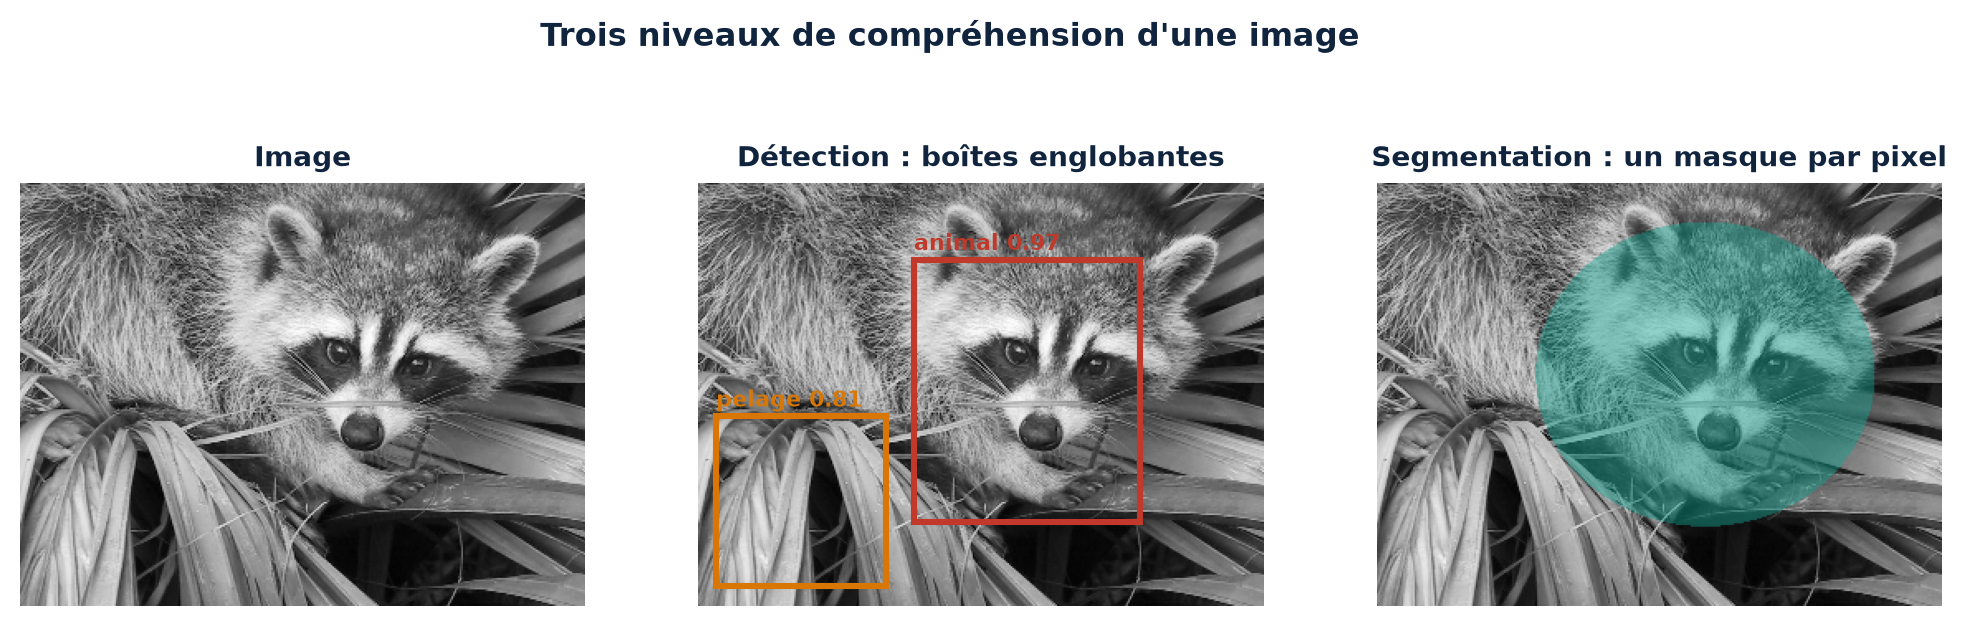
\includegraphics[width=.92\textwidth]{j01_detection_segmentation.png}\end{center}\end{frame}

\begin{frame}{Ce que produit un détecteur}
\begin{columns}[t]
\begin{column}{0.52\textwidth}
\begin{itemize}
  \item Un détecteur renvoie une \textbf{liste de détections}. Chaque détection
  contient :
  \begin{itemize}
    \item une \textbf{boîte englobante} (\emph{bounding box}) : les coordonnées
    du rectangle qui entoure l'objet ;
    \item une \textbf{classe} : la catégorie reconnue ;
    \item un \textbf{score de confiance} : un nombre entre 0 et 1.
  \end{itemize}
  \item Deux écritures courantes pour la boîte :
  \begin{itemize}
    \item coin haut-gauche $(x_1, y_1)$ et coin bas-droit $(x_2, y_2)$ ;
    \item centre $(x_c, y_c)$ plus largeur $w$ et hauteur $h$.
  \end{itemize}
\end{itemize}
\end{column}
\begin{column}{0.46\textwidth}
\begin{ebox}[Exemple de détection]
\py{(classe='chien', score=0.91,\\ x1=42, y1=77, x2=210, y2=290)}
\medskip

Le \emph{score de confiance} n'est pas une probabilité de justesse : c'est un
nombre \emph{appris} qui sert à \textbf{trier} les détections.
\end{ebox}

\end{column}
\end{columns}
% [fix] bloc deplace
\end{frame}
\begin{frame}{Ce que produit un détecteur (suite)}
\begin{wbox}[Une image, plusieurs objets]
Une image contient souvent \emph{plusieurs} objets : le détecteur doit donc
rendre une liste de longueur variable, pas une sortie de taille fixe.
\end{wbox}
\end{frame}

\begin{frame}{L'IoU : mesurer le recouvrement de deux boîtes}
\begin{columns}[t]
\begin{column}{0.50\textwidth}
\begin{itemize}
  \item Deux boîtes ne coïncident presque jamais exactement.
  \item L'\textbf{IoU} (\emph{Intersection over Union}) mesure leur recouvrement :
\end{itemize}
\[
\mathrm{IoU}(A,B)=\frac{|A\cap B|}{|A\cup B|}
\]
\begin{itemize}
  \item $\mathrm{IoU}=0$ : boîtes disjointes ; $\mathrm{IoU}=1$ : boîtes identiques.
  \item L'IoU sert à \emph{toutes} les étapes : définir une bonne détection,
  comparer au seuil de validation, et supprimer les doublons.
\end{itemize}
\end{column}
\begin{column}{0.48\textwidth}
\begin{kbox}[Le rôle de l'IoU]
C'est la \textbf{métrique de référence} de la localisation. Sans elle, impossible
de dire si une boîte prédite est « correcte », ni si deux détections désignent
le même objet.
\end{kbox}
\vspace{1mm}
\begin{ebox}[Un seuil de référence]
Pour juger une détection correcte on compare l'IoU à un seuil ; le seuil usuel
de référence est $\mathrm{IoU} \ge 0{,}5$ : la prédiction doit recouvrir au moins
la moitié de l'union pour être acceptée.
\end{ebox}
\end{column}
\end{columns}
\end{frame}

\begin{frame}{La suppression des non-maxima (NMS)}
\begin{columns}[t]
\begin{column}{0.50\textwidth}
\begin{itemize}
  \item Un détecteur produit \textbf{beaucoup} de boîtes : plusieurs versions
  un peu décalées du même objet.
  \item La \textbf{suppression des non-maxima} (NMS) élimine ces doublons.
  \item Principe :
  \begin{enumerate}
    \item trier les boîtes par score décroissant ;
    \item garder la meilleure ;
    \item supprimer toutes celles dont l'IoU avec elle dépasse un seuil ;
    \item répéter sur ce qui reste.
  \end{enumerate}
\end{itemize}
\end{column}
\begin{column}{0.48\textwidth}
\begin{kbox}[Le seuil de la NMS]
Dans ce cours, le seuil de recouvrement utilisé pour la NMS est
$\mathrm{IoU} = 0{,}45$. Une boîte recouvrant la boîte gardée à plus de
$45 \ \%$ est considérée comme un doublon.
\end{kbox}
\begin{wbox}[Deux objets, gardés tous les deux]
Deux objets réellement distincts ont un IoU \emph{faible} : ils survivent
tous les deux à la NMS. Le seuil arbitre entre \emph{doublon} et \emph{voisins}.
\end{wbox}
\end{column}
\end{columns}
\end{frame}

\begin{frame}[fragile]{La NMS en Python}
\begin{columns}[t]
\begin{column}{0.50\textwidth}
\begin{codebox}[Suppression des non-maxima]
\begin{lstlisting}
import numpy as np

def iou(a, b):
    x1 = max(a[0], b[0]); y1 = max(a[1], b[1])
    x2 = min(a[2], b[2]); y2 = min(a[3], b[3])
    inter = max(0, x2-x1) * max(0, y2-y1)
    aire_a = (a[2]-a[0]) * (a[3]-a[1])
    aire_b = (b[2]-b[0]) * (b[3]-b[1])
    union = aire_a + aire_b - inter
    return inter / union

def nms(boxes, scores, seuil=0.45):
    ordre = np.argsort(scores)[::-1]
    gardees = []
    while len(ordre) > 0:
        i = ordre[0]
        gardees.append(i)
        reste = [j for j in ordre[1:]
                  if iou(boxes[i], boxes[j]) <= seuil]
        ordre = np.array(reste)
    return gardees
\end{lstlisting}
\end{codebox}
\end{column}
\begin{column}{0.48\textwidth}
\begin{itemize}
  \item Le seuil $\mathrm{IoU} = 0{,}45$ est passé en argument de
  \py{nms}.
  \item L'algorithme est glouton : on garde toujours la meilleure boîte
  restante.
  \item Coût : dominé par le calcul des IoU entre boîtes restantes.
  \item La NMS est une étape \emph{post-traitement} : elle ne dépend pas
  de l'architecture du réseau.
\end{itemize}

\end{column}
\end{columns}
% [fix] bloc deplace
\end{frame}
\begin{frame}{La NMS en Python (suite)}
\begin{wbox}[Piège classique]
Un seuil de NMS \emph{trop bas} fusionne des objets voisins distincts ; un seuil
\emph{trop haut} laisse passer des doublons.
\end{wbox}
\end{frame}

\begin{frame}{Les deux familles de détecteurs}
\begin{columns}[t]
\begin{column}{0.46\textwidth}
\centering
\end{column}
\begin{column}{0.51\textwidth}
\begin{ebox}[En deux étapes]
\textbf{R-CNN}, \textbf{Faster R-CNN}. Une première étape propose des
\emph{régions}, une seconde les classe et raffine les boîtes. Précision élevée,
calcul plus lourd.
\end{ebox}
\begin{ebox}[En une étape]
\textbf{YOLO}, \textbf{SSD}. Le réseau prédit directement boîtes et classes
en \emph{un seul passage} sur l'image. Très rapide, adapté au temps réel.
\end{ebox}
\end{column}
\end{columns}
\vspace{0.5mm}
\begin{kbox}[L'arbitrage]
Deux étapes favorisent la précision ; une étape favorise la vitesse. Le choix
dépend de la contrainte temps réel de l'application.
\end{kbox}
% [fix] figure sortie
\end{frame}

\begin{frame}{Les deux familles de détecteurs --- la figure}% [fix] figure sortie
\end{frame}

\begin{frame}{Les deux familles de détecteurs --- la figure --- la figure}\begin{center}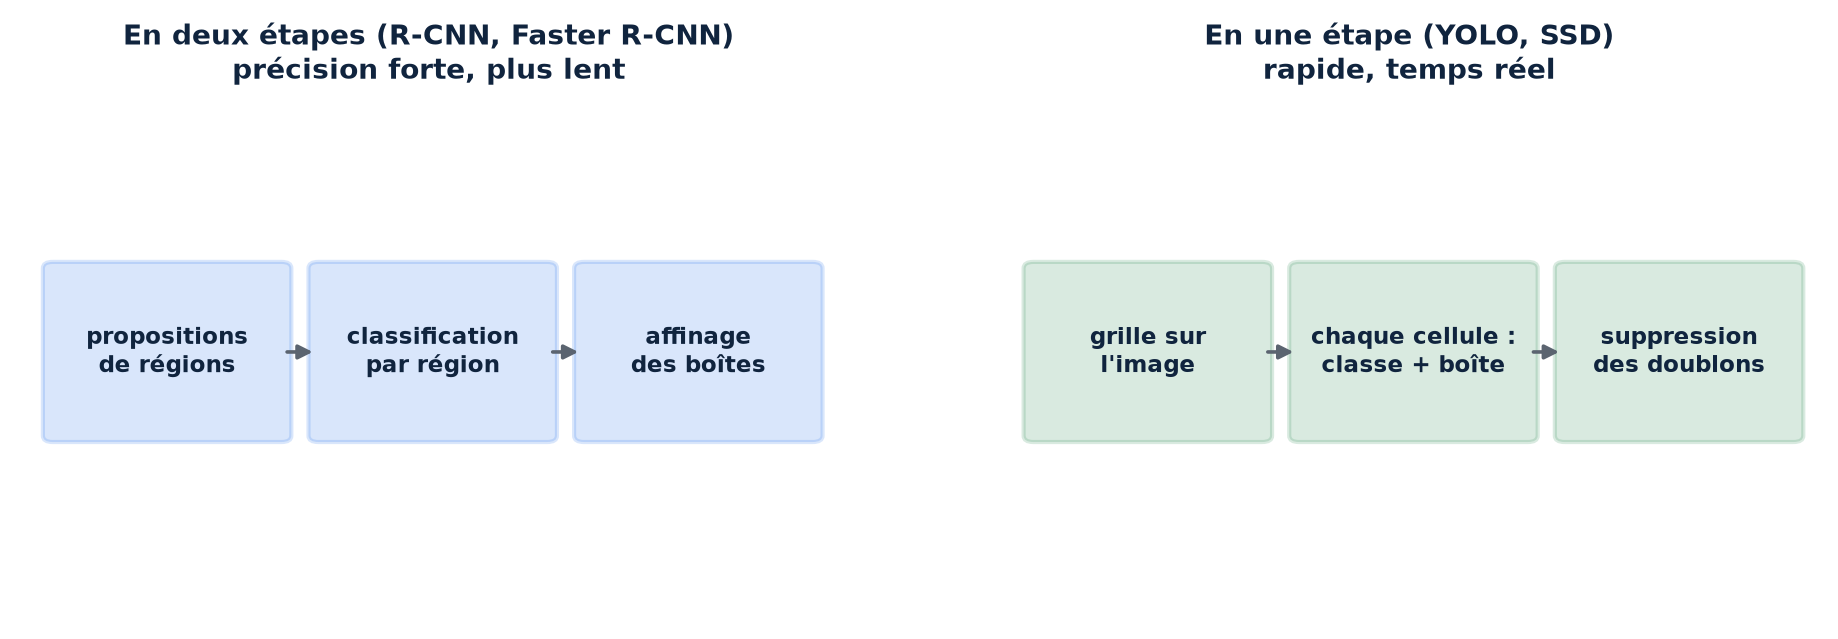
\includegraphics[width=.92\textwidth]{j03_une_deux_etapes.png}\end{center}\end{frame}

\begin{frame}{Une étape ou deux : le tableau de synthèse}
\begin{center}
\begin{tabular}{@{}p{4.2cm}p{4.7cm}p{4.7cm}@{}}
\toprule
 & \textbf{Deux étapes} & \textbf{Une étape} \\
\midrule
Modèles & R-CNN, Faster R-CNN & YOLO, SSD \\
Principe & proposer des régions, puis classer & prédire boîtes et classes d'un coup \\
Points forts & détection précise des petits objets & très rapide, temps réel \\
Points faibles & plus lent, pipeline plus complexe & moins précis sur très petits objets \\
\bottomrule
\end{tabular}
\end{center}
\vspace{1mm}

% [fix] bloc deplace
\end{frame}
\begin{frame}{Une étape ou deux : le tableau de synthèse (suite)}

% [fix] bloc deplace
\end{frame}
\begin{frame}{Une étape ou deux : le tableau de synthè… (suite)}
\begin{wbox}[Vocabulaire à retenir]
\emph{Région proposée} : une zone candidate renvoyée par le réseau avant
classification. \emph{Détection dense} : une prédiction à chaque position de
la carte, sans étape de proposition.
\end{wbox}
\end{frame}

\begin{frame}{La segmentation : trois niveaux}
\begin{columns}[t]
\begin{column}{0.52\textwidth}
\centering
\end{column}
\begin{column}{0.45\textwidth}
\begin{itemize}
  \item \textbf{Ségmentation sémantique} : chaque pixel reçoit une classe ;
  deux objets de même classe ne sont pas distingués.
  \item \textbf{Segmentation par instance} : chaque \emph{objet} individuel
  reçoit sa propre étiquette (vache 1, vache 2, \dots).
  \item \textbf{Segmentation panoptique} : unifie les deux ; chaque pixel est
  étiqueté soit comme une \emph{chose} (objet comptable), soit comme une
  \emph{matière} (sans forme : ciel, route, herbe).
\end{itemize}
\end{column}
\end{columns}
\vspace{0.5mm}
\begin{kbox}[La bonne question]
« Combien d'objets, et séparés ? » $\rightarrow$ par instance.
« Quelle est la nature de chaque pixel ? » $\rightarrow$ sémantique.
« Les deux à la fois ? » $\rightarrow$ panoptique.
\end{kbox}
% [fix] figure sortie
\end{frame}

\begin{frame}{La segmentation : trois niveaux --- la figure}\begin{center}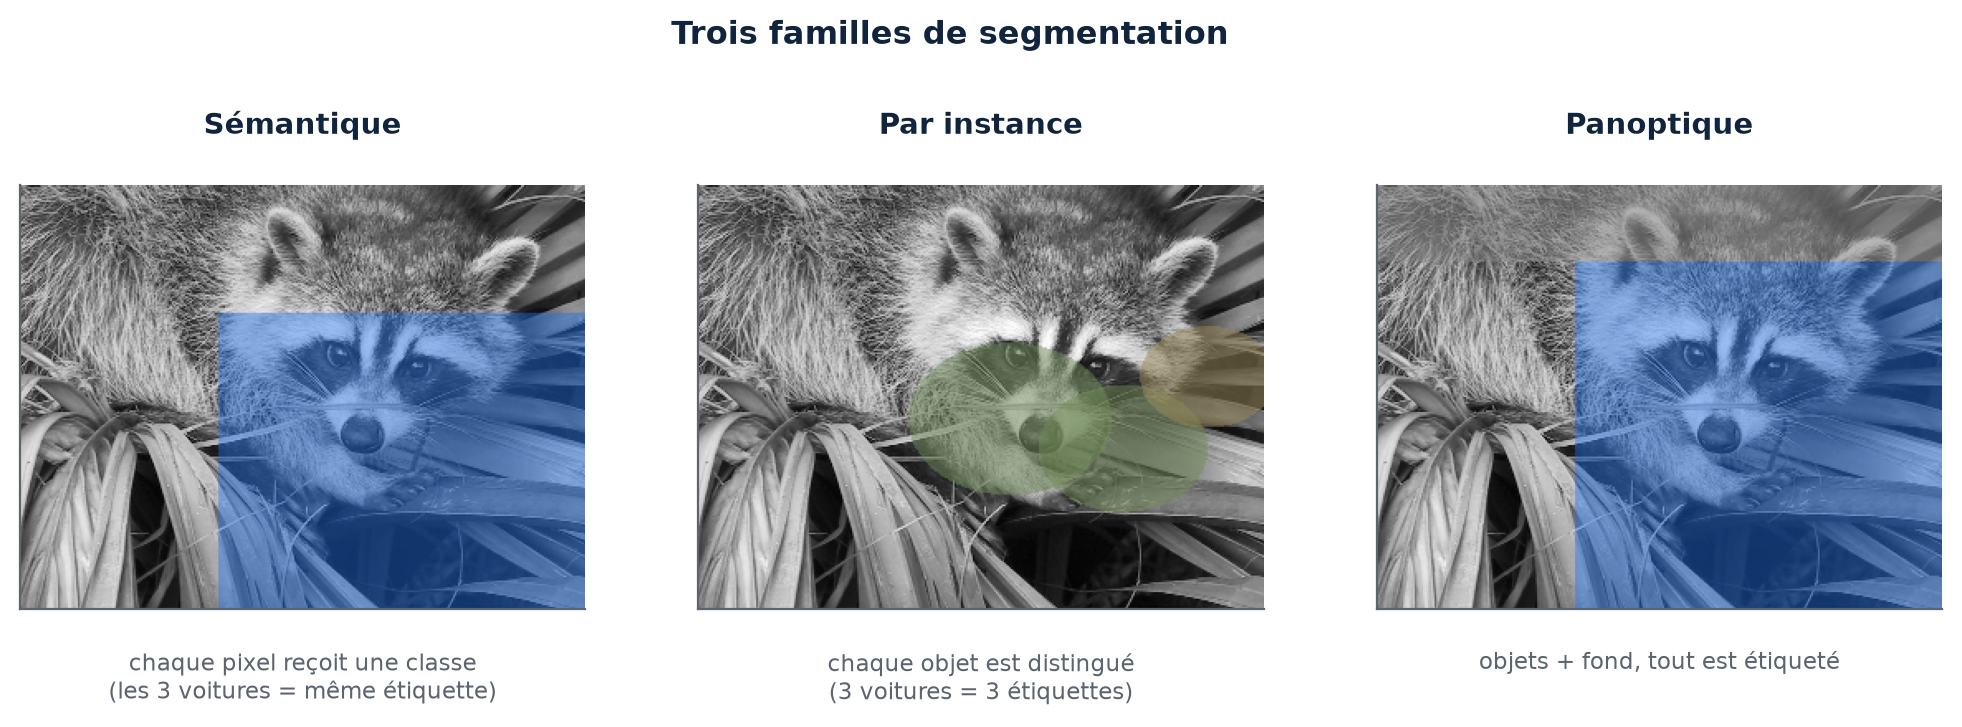
\includegraphics[width=.92\textwidth]{j02_trois_segmentations.png}\end{center}\end{frame}

\begin{frame}{Sémantique, instance, panoptique : définitions exactes}
\begin{center}
\begin{tabular}{@{}p{3.0cm}p{5.0cm}p{5.4cm}@{}}
\toprule
\textbf{Type} & \textbf{Définition} & \textbf{Sortie typique} \\
\midrule
Sémantique & une classe par pixel, sans séparer les instances & une carte de classes \\
Par instance & une étiquette distincte pour chaque objet, plus le fond & masques d'objets \\
Panoptique & chaque pixel : classe de \emph{chose} (avec instance) ou de \emph{matière} & étiquettes unifiées \\
\bottomrule
\end{tabular}
\end{center}
\vspace{1mm}
\begin{columns}[t]
\begin{column}{0.48\textwidth}
\begin{ebox}[Applications]
Imagerie médicale (tumeurs, organes), conduite autonome (route, piétons,
véhicules), télédétection.
\end{ebox}
\end{column}
\begin{column}{0.48\textwidth}

\end{column}
\end{columns}
% [fix] bloc deplace
\end{frame}
\begin{frame}{Sémantique, instance, panoptique : défin… (suite)}
\begin{wbox}[Choses vs matières]
Les \emph{choses} sont dénombrables (voitures, personnes) ; les \emph{matières}
ne le sont pas (ciel, eau). La segmentation panoptique traite les deux.
\end{wbox}
\end{frame}

\begin{frame}{L'architecture encodeur--décodeur}
\begin{columns}[t]
\begin{column}{0.52\textwidth}
\centering
\end{column}
\begin{column}{0.45\textwidth}
\begin{itemize}
  \item Une segmentation doit \textbf{rétablir la résolution} de l'image
  d'entrée : la sortie a la taille de l'entrée.
  \item L'\textbf{encodeur} réduit la résolution et augmente le nombre de
  canaux : il résume le contenu.
  \item Le \textbf{décodeur} fait l'inverse : il remonte la résolution
  (par ex.\ déconvolution ou interpolation) pour retrouver une carte dense.
  \item \textbf{U-Net} est l'archétype de ce schéma, en forme de « U ».
\end{itemize}
\end{column}
\end{columns}
\vspace{0.5mm}
\begin{kbox}[Le principe]
En descendant, on gagne du \emph{contexte} mais on perd la \emph{position fine}.
En remontant, on la retrouve : d'où l'intérêt des connexions sautées.
\end{kbox}
% [fix] figure sortie
\end{frame}

\begin{frame}{L'architecture encodeur--décodeur --- la figure}\begin{center}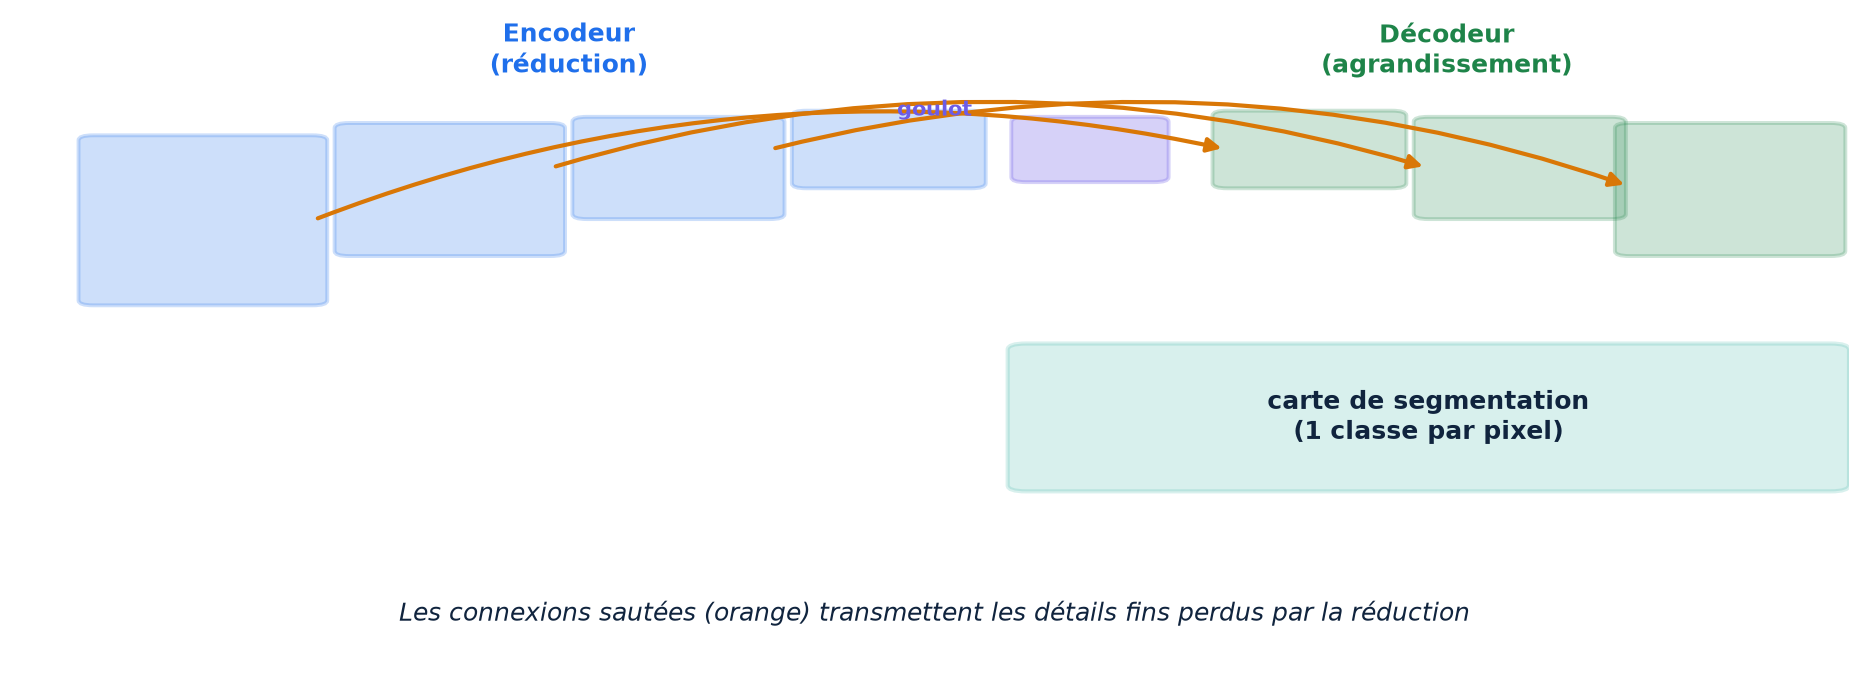
\includegraphics[width=.92\textwidth]{j04_unet.png}\end{center}\end{frame}

\begin{frame}{Les connexions sautées de U-Net}
\begin{columns}[t]
\begin{column}{0.48\textwidth}
\begin{itemize}
  \item À chaque niveau de l'encodeur, les cartes de caractéristiques sont
  \textbf{recopiées} vers le niveau correspondant du décodeur.
  \item U-Net comporte \textbf{3 connexions sautées} reliant encodeur
  et décodeur.
  \item Ces sauts apportent au décodeur l'information spatiale précise
  (contours, positions) que la descente avait résumée.
\end{itemize}
\end{column}
\begin{column}{0.48\textwidth}
\begin{kbox}[Pourquoi cela marche]
Le décodeur, seul, ne dispose que de résumés \emph{grossiers}. Grâce aux sauts,
il combine \emph{contexte} (venu du bas) et \emph{détail} (venu de l'encodeur) :
les frontières entre objets deviennent nettes.
\end{kbox}

\end{column}
\end{columns}
% [fix] bloc deplace
\end{frame}
\begin{frame}{Les connexions sautées de U-Net (suite)}
\begin{wbox}[À ne pas confondre]
Connexion sautée de U-Net (concaténation de cartes entre encodeur et décodeur)
et connexion résiduelle de ResNet (addition d'une identité dans un bloc) :
même mot, buts différents.
\end{wbox}
\end{frame}
